% Measuring Clutch Performance in Soccer When the Result Is on the Line
% Springer CCIS / LNCS format. Every number comes from numbers.tex, written by pipeline/s14_claims.py.
% Main figure: figures/method.pdf, a vector conversion of figures/method.svg.
\documentclass[runningheads]{llncs}
\usepackage[T1]{fontenc}
\usepackage[utf8]{inputenc}
\usepackage{amsmath,amssymb}
\usepackage{graphicx}
\usepackage{placeins}
\usepackage{booktabs}
\usepackage{marvosym}
\usepackage{url}
\usepackage[hidelinks]{hyperref}
\usepackage{color}
\renewcommand\UrlFont{\color{blue}\rmfamily}
\urlstyle{rm}
% Keep words whole at line endings throughout the paper, including references.
\hyphenpenalty=10000
\exhyphenpenalty=10000
\emergencystretch=3em
% Allow URL wrapping at separators, never in the middle of a name or word.
\def\UrlBreaks{\do\/\do\:}
\def\UrlBigBreaks{\do\/\do\:}
\newcommand{\scoreMatch}{99.97}
\newcommand{\nMatches}{1,826}
\newcommand{\nActions}{2.32 million}
\newcommand{\nActionsExact}{2,320,430}
\newcommand{\nGoals}{4,793}
\newcommand{\nOwnGoals}{153}
\newcommand{\aucScores}{.77}
\newcommand{\aucConcedes}{.75}
\newcommand{\psxgAuc}{.82}
\newcommand{\stakesRps}{0.154}
\newcommand{\stakesBias}{0.001}
\newcommand{\realCost}{1.58}
\newcommand{\realGain}{0.23}
\newcommand{\modelCost}{1.56}
\newcommand{\modelGain}{0.23}
\newcommand{\costGainDiff}{1.35}
\newcommand{\costGainLow}{1.25}
\newcommand{\costGainHigh}{1.44}
\newcommand{\levelGain}{1.58}
\newcommand{\levelCost}{0.96}
\newcommand{\levelModelGain}{1.58}
\newcommand{\levelModelCost}{0.98}
\newcommand{\downGain}{0.96}
\newcommand{\downCost}{0.12}
\newcommand{\downModelGain}{0.95}
\newcommand{\downModelCost}{0.13}
\newcommand{\nCells}{33}
\newcommand{\rhoCost}{.99}
\newcommand{\rhoCostLow}{.98}
\newcommand{\rhoCostHigh}{1.00}
\newcommand{\maeCost}{.05}
\newcommand{\slopeCost}{.93}
\newcommand{\rhoGain}{.99}
\newcommand{\maeGain}{.05}
\newcommand{\rhoTotal}{.99}
\newcommand{\rhoTotalLow}{.95}
\newcommand{\rhoTotalHigh}{.99}
\newcommand{\rhoTotalSO}{.72}
\newcommand{\rhoTotalSOLow}{.69}
\newcommand{\rhoTotalSOHigh}{.74}
\newcommand{\rhoCostSO}{.33}
\newcommand{\rhoGainSO}{.98}
\newcommand{\rhoShiftSO}{.98}
\newcommand{\rhoShiftL}{1.00}
\newcommand{\nShiftCells}{24}
\newcommand{\kickHomeW}{1.52}
\newcommand{\kickHomeReal}{1.61}
\newcommand{\kickAwayW}{1.20}
\newcommand{\kickAwayReal}{1.15}
\newcommand{\ledgerMatchSlope}{1.12}
\newcommand{\ledgerMatchR}{.91}
\newcommand{\ledgerSeasonSlope}{1.09}
\newcommand{\ledgerSeasonR}{.975}
\newcommand{\ledgerSeasonRGd}{.965}
\newcommand{\ledgerSeasonRVaep}{.962}
\newcommand{\ledgerMatchRGd}{.84}
\newcommand{\ledgerMatchRVaep}{.83}
\newcommand{\ledgerTeams}{98}
\newcommand{\creditLow}{2.4}
\newcommand{\creditHigh}{2.6}
\newcommand{\weightTwo}{2.53}
\newcommand{\weightSO}{0.52}
\newcommand{\weightRatio}{4.8}
\newcommand{\nQualified}{1,634}
\newcommand{\meanCPIF}{.16}
\newcommand{\meanCPIM}{.15}
\newcommand{\meanCPID}{.11}
\newcommand{\meanCPIG}{.09}
\newcommand{\messiCPI}{.64}
\newcommand{\messiLow}{.43}
\newcommand{\messiHigh}{.86}
\newcommand{\messiTotal}{21.2}
\newcommand{\relCPIF}{.32}
\newcommand{\relVaepF}{.42}
\newcommand{\disCPIF}{.27}
\newcommand{\relCPIM}{.48}
\newcommand{\relVaepM}{.54}
\newcommand{\disCPIM}{.44}
\newcommand{\relCPID}{.41}
\newcommand{\relVaepD}{.48}
\newcommand{\disCPID}{.38}
\newcommand{\relCPIG}{.17}
\newcommand{\relVaepG}{.21}
\newcommand{\disCPIG}{.03}
\newcommand{\relSaved}{.24}
\newcommand{\disSaved}{.10}
\newcommand{\abilityLow}{79}
\newcommand{\abilityHigh}{100}
\newcommand{\deliveryLow}{8}
\newcommand{\deliveryHigh}{21}
\newcommand{\exposureMax}{8}
\newcommand{\deliveryRhoLow}{$-$.05}
\newcommand{\deliveryRhoHigh}{.05}
\newcommand{\corrVaepF}{.91}
\newcommand{\corrGaF}{.72}
\newcommand{\relSOF}{.35}
\newcommand{\relGoalsF}{.52}
\newcommand{\corrVaepM}{.88}
\newcommand{\corrGaM}{.57}
\newcommand{\relSOM}{.45}
\newcommand{\relGoalsM}{.58}
\newcommand{\corrVaepD}{.87}
\newcommand{\corrGaD}{.49}
\newcommand{\relSOD}{.39}
\newcommand{\relGoalsD}{.41}
\newcommand{\corrVaepG}{.10}
\newcommand{\corrGaG}{$-$.05}
\newcommand{\relSOG}{.44}
\newcommand{\relDefendD}{.24}
\newcommand{\disDefendD}{.18}
\newcommand{\leadDefenders}{J. Alonso (1.02), B. Dibassy (0.78), Juanpe (0.69)}
\newcommand{\riseDefenders}{I. Sylla (57 to 28), J. Koundé (62 to 34), Bartra (69 to 48)}
\newcommand{\goalsMoreno}{15}
\newcommand{\gptsMoreno}{11.6}
\newcommand{\ppgMoreno}{.78}
\newcommand{\decidedMoreno}{7}
\newcommand{\goalsRonaldo}{23}
\newcommand{\gptsRonaldo}{11.4}
\newcommand{\ppgRonaldo}{.50}
\newcommand{\decidedRonaldo}{30}
\newcommand{\goalsAubameyang}{19}
\newcommand{\gptsAubameyang}{5.8}
\newcommand{\ppgAubameyang}{.30}
\newcommand{\decidedAubameyang}{37}
\newcommand{\goalsZapata}{11}
\newcommand{\gptsZapata}{9.3}
\newcommand{\ppgZapata}{.85}
\newcommand{\decidedZapata}{9}
\newcommand{\goalsAguero}{17}
\newcommand{\gptsAguero}{5.7}
\newcommand{\ppgAguero}{.34}
\newcommand{\decidedAguero}{47}
\newcommand{\goalsSalah}{31}
\newcommand{\gptsSalah}{15.9}
\newcommand{\ppgSalah}{.51}
\newcommand{\decidedSalah}{19}
\newcommand{\costlyAllOwn}{12}
\newcommand{\skriniarCost}{1.52}
\newcommand{\skriniarMinute}{87}
\newcommand{\medianShots}{144}
\newcommand{\savedGea}{11.1}
\newcommand{\preventedGea}{16.7}
\newcommand{\savedOblak}{11.0}
\newcommand{\preventedOblak}{11.1}
\newcommand{\savedAlisson}{11.1}
\newcommand{\preventedAlisson}{16.0}
\newcommand{\savedPope}{10.0}
\newcommand{\preventedPope}{13.5}
\newcommand{\savedCech}{$-$4.5}
\newcommand{\preventedCech}{$-$3.5}
\newcommand{\marginBarca}{14}
\newcommand{\paaBarca}{15.8}
\newcommand{\marginJuve}{4}
\newcommand{\paaJuve}{6.3}
\newcommand{\marginLille}{1}
\newcommand{\paaLille}{5.2}
\newcommand{\cutHigh}{1.71}
\newcommand{\cutLow}{0.98}
\newcommand{\baseCompletion}{83.3}
\newcommand{\nPasses}{1.54 million}
\newcommand{\qCompletion}{1.0}
\newcommand{\qProgress}{0.53}
\newcommand{\qValuePct}{31}
\newcommand{\meanValue}{3.5}
\newcommand{\xSideCompletion}{3.3}
\newcommand{\xSideProgress}{0.94}
\newcommand{\xRoute}{0.6}
\newcommand{\nTakenOff}{3,307}
\newcommand{\nBroughtOn}{2,771}
\newcommand{\orOffUpDef}{.88}
\newcommand{\orOffUpDefLow}{0.83}
\newcommand{\orOffUpDefHigh}{0.94}
\newcommand{\orOffUpAtt}{1.03}
\newcommand{\orOffUpAttLow}{0.98}
\newcommand{\orOffUpAttHigh}{1.09}
\newcommand{\orOffDownDef}{1.00}
\newcommand{\orOffDownDefLow}{0.96}
\newcommand{\orOffDownDefHigh}{1.07}
\newcommand{\orOffDownAtt}{.84}
\newcommand{\orOffDownAttLow}{0.78}
\newcommand{\orOffDownAttHigh}{0.89}
\newcommand{\orOnUpDef}{1.00}
\newcommand{\orOnUpDefLow}{0.95}
\newcommand{\orOnUpDefHigh}{1.06}
\newcommand{\orOnUpAtt}{.96}
\newcommand{\orOnUpAttLow}{0.91}
\newcommand{\orOnUpAttHigh}{1.03}
\newcommand{\orOnDownDef}{.85}
\newcommand{\orOnDownDefLow}{0.78}
\newcommand{\orOnDownDefHigh}{0.92}
\newcommand{\orOnDownAtt}{1.22}
\newcommand{\orOnDownAttLow}{1.13}
\newcommand{\orOnDownAttHigh}{1.32}
\newcommand{\pickUp}{43.7}
\newcommand{\pickUpChance}{43.5}
\newcommand{\pickDown}{51.7}
\newcommand{\pickDownChance}{44.0}
\newcommand{\pickUpN}{954}
\newcommand{\pickDownN}{733}
\newcommand{\mirrorAuc}{.75}
\newcommand{\baseAuc}{.77}
\newcommand{\mirrorKeeper}{$-$.04}
\newcommand{\baseKeeper}{.09}
\newcommand{\baseForward}{.16}
\newcommand{\noBaseForward}{.20}
\newcommand{\noBaseTopMid}{5}
\newcommand{\sensRhoMin}{.95}
\newcommand{\sensTopMin}{7}
\newcommand{\strengthRhoMin}{.99}
\newcommand{\thresholdLow}{5}
\newcommand{\thresholdHigh}{8}
\newcommand{\goalLevelLateV}{1.43}
\newcommand{\goalUpLateV}{.18}
\newcommand{\goalVaepLow}{.86}
\newcommand{\goalVaepHigh}{.87}
\newcommand{\shareLowVaep}{22}
\newcommand{\shareLowCpi}{5}
\newcommand{\shareTopVaep}{23}
\newcommand{\shareTopCpi}{37}
\newcommand{\sharedTopLow}{4}
\newcommand{\sharedTopHigh}{6}
\newcommand{\moveLow}{21}
\newcommand{\moveHigh}{43}
\newcommand{\beyondLow}{.01}
\newcommand{\beyondHigh}{.12}
\newcommand{\caseGoalsM}{0.45}
\newcommand{\caseGoalsR}{0.46}
\newcommand{\casePassM}{0.18}
\newcommand{\casePassR}{0.04}
\newcommand{\caseMissM}{0.10}
\newcommand{\caseMissR}{0.22}
\newcommand{\ronaldoRank}{32}
\newcommand{\ronaldoCPI}{.31}
\newcommand{\ronaldoShrunkRank}{67}
\newcommand{\nForwards}{320}
\newcommand{\messiActions}{82}
\newcommand{\ronaldoActions}{45}
\newcommand{\caseAhead}{97}
\newcommand{\caseLow}{$-$.01}
\newcommand{\caseHigh}{.64}
\newcommand{\exAMatch}{Crystal Palace v Manchester United}
\newcommand{\exAMinute}{91}
\newcommand{\exAScore}{2--2}
\newcommand{\exAPs}{0.988}
\newcommand{\exAPc}{0.005}
\newcommand{\exAPrevPs}{0.012}
\newcommand{\exAPrevPc}{0.010}
\newcommand{\exAdPs}{0.976}
\newcommand{\exAdPc}{$-$0.005}
\newcommand{\exALp}{1.673}
\newcommand{\exALm}{0.970}
\newcommand{\exAV}{1.638}
\newcommand{\exAVaep}{0.981}
\newcommand{\exAType}{shot}
\newcommand{\exAPlayer}{N. Mati\'{c}}
\newcommand{\exBMatch}{Lille v Toulouse}
\newcommand{\exBMinute}{92}
\newcommand{\exBScore}{1--0}
\newcommand{\exBPs}{0.004}
\newcommand{\exBPc}{0.020}
\newcommand{\exBPrevPs}{0.021}
\newcommand{\exBPrevPc}{0.429}
\newcommand{\exBdPs}{$-$0.017}
\newcommand{\exBdPc}{$-$0.409}
\newcommand{\exBLp}{0.166}
\newcommand{\exBLm}{1.629}
\newcommand{\exBV}{0.663}
\newcommand{\exBVaep}{0.392}
\newcommand{\exBType}{clearance}
\newcommand{\exBPlayer}{J. Alonso}
\newcommand{\wxN}{6}
\newcommand{\wxFt}{0.199}
\newcommand{\wxFo}{0.132}
\newcommand{\wxTt}{0.0362}
\newcommand{\wxTo}{0.0234}
\newcommand{\wxWin}{0.892}
\newcommand{\wxDraw}{0.101}
\newcommand{\wxW}{2.779}
\newcommand{\wxWup}{2.987}
\newcommand{\wxWdown}{1.241}
\newcommand{\wxLp}{0.209}
\newcommand{\wxLm}{1.537}
\newcommand{\wxPgoal}{0.199}
\newcommand{\lrBzero}{-2.083}
\newcommand{\lrBg}{0.112}
\newcommand{\lrBn}{0.0542}
\newcommand{\lrBnn}{-0.000265}
\newcommand{\lrBh}{0.261}
\newcommand{\nFeatures}{64}
\newcommand{\eceMax}{1.16}
\newcommand{\psxgGoals}{4,786}
\newcommand{\psxgPred}{4,784}
\newcommand{\psxgShots}{15,646}
\newcommand{\psxgBrier}{0.151}
\newcommand{\qPlayersMatches}{50,367}
\newcommand{\qOffUp}{1,684}
\newcommand{\qOffDown}{1,623}
\newcommand{\tabLeaders}{%
Forwards & L. Messi & .64 (.43, .86) & 21.2 & .24 & 48\% & 1 \\
 & Neymar & .48 (.29, .67) & 9.5 & .22 & 31\% & 2 \\
 & L. Bailey & .46 (.26, .69) & 11.3 & .21 & 23\% & 18 \\
\midrule
Midfielders & N. Fekir & .48 (.26, .71) & 13.1 & .19 & 13\% & 1 \\
 & E. Giaccherini & .46 (.20, .86) & 5.0 & .16 & 5\% & 21 \\
 & R. Mahrez & .45 (.30, .60) & 14.7 & .23 & 37\% & 5 \\
\midrule
Defenders & J. Roussillon & .30 (.18, .42) & 6.2 & .15 & 19\% & 8 \\
 & L. Dubois & .29 (.21, .39) & 9.8 & .18 & 45\% & 13 \\
 & Z. Feddal & .28 (.07, .55) & 4.0 & .12 & 4\% & 41 \\
\midrule
Goalkeepers & N. Pope & .42 (.24, .63) & 14.6 & .11 & 27\% & 8 \\
 & Alisson & .39 (.18, .59) & 14.5 & .10 & 22\% & 18 \\
 & A. Meret & .37 (.14, .59) & 4.7 & .10 & 18\% & 120 \\
}
\newcommand{\tabMoments}{%
\multicolumn{5}{@{}l}{\textit{Most valuable}} \\
Thomas & Deportivo La Coruña v Atlético Madrid 0--1 & 91$'$ & 0--0 & +1.66 \\
M. Sylla & Caen v Monaco 1--2 & 91$'$ & 1--1 & +1.65 \\
B. Srarfi & Toulouse v Nice 1--2 & 91$'$ & 1--1 & +1.65 \\
M. Destro & Chievo v Bologna 2--3 & 90$'$ & 2--2 & +1.65 \\
\midrule
\multicolumn{5}{@{}l}{\textit{Most costly}} \\
S. Yago & Toulouse v Strasbourg 2--2 & 94$'$ & 2--1 & $-$1.57 \\
K. Vogt & Hoffenheim v Augsburg 2--2 & 89$'$ & 2--1 & $-$1.52 \\
M. \v{S}kriniar & Internazionale v Juventus 2--3 & 87$'$ & 2--1 & $-$1.52 \\
M. Batshuayi & Tottenham Hotspur v Chelsea 1--2 & 81$'$ & 1--0 & $-$1.46 \\
}
\newcommand{\tabPressure}{%
Pass completion, pp & $-$1.03 ($-$1.71, $-$0.35) & 0.009 \\
Action value, $\times 10^{-3}$ & $-$1.07 ($-$1.63, $-$0.51) & 0.001 \\
Pass forward progress, m & +0.53 (+0.26, +0.79) & 0.001 \\
Completion: home $\times$ stakes & +0.15 ($-$0.56, +0.85) & 1.00 \\
Completion: age (per 5 y) $\times$ stakes & $-$0.09 ($-$0.44, +0.27) & 1.00 \\
\midrule
\multicolumn{3}{@{}l}{\textit{Exploratory: which side of the stakes is larger}} \\
Completion, pp: scoring side & +0.07 ($-$0.63, +0.78) & -- \\
Completion, pp: conceding side & $-$3.27 ($-$4.13, $-$2.40) & -- \\
Progress, m: scoring side & +0.32 (+0.04, +0.60) & -- \\
Progress, m: conceding side & +0.94 (+0.62, +1.26) & -- \\
Value, $\times 10^{-3}$: scoring side & $-$1.51 ($-$2.08, $-$0.94) & -- \\
Value, $\times 10^{-3}$: conceding side & $-$0.31 ($-$0.99, +0.38) & -- \\
}
\newcommand{\tabSensitivity}{%
another seed & 1.00 & .99 & .99 & 1.00 & 10, 9, 8, 10 \\
another booster & .99 & .98 & .96 & 1.00 & 10, 7, 9, 10 \\
window of 5 actions & .98 & .96 & .95 & .99 & 9, 7, 7, 10 \\
window of 15 actions & .99 & .99 & .97 & 1.00 & 10, 9, 7, 9 \\
team strength in the stakes & .99 & .99 & .99 & 1.00 & 8, 8, 7, 10 \\
}
\newcommand{\tabChoices}{%
Away actions left mirrored & .97 & .94 & .84 & .95 & 10, 6, 6, 9 \\
No penalty, corner baselines & .91 & .92 & .98 & 1.00 & 9, 5, 6, 10 \\
}
\newcommand{\tabGoalValues}{%
Level, 85$'$+ & 116 & .87 & 1.43 \\
One down, 85$'$+ & 94 & .90 & .87 \\
Level, first 15$'$ & 486 & .89 & .69 \\
One up, 85$'$+ & 87 & .86 & .18 \\
Three or more up, 60$'$+ & 162 & .83 & .00 \\
}
\newcommand{\tabMovers}{%
P. Aubameyang & Fwd & Borussia Dortmund & 42 & 156 \\
P. Crouch & Fwd & Stoke City & 205 & 85 \\
Paulinho & Mid & Barcelona & 118 & 465 \\
Jesús Navas & Mid & Sevilla & 449 & 115 \\
A. Robertson & Def & Liverpool & 108 & 449 \\
Laguardia & Def & Deportivo Alavés & 281 & 32 \\
}
\newcommand{\tabCase}{%
Goals & 0.45 & 0.46 & $-$0.01 \\
Passes and crosses & 0.18 & 0.04 & 0.14 \\
Missed shots & $-$0.10 & $-$0.22 & 0.12 \\
Dribbles and take-ons & 0.07 & 0.04 & 0.03 \\
Other actions & 0.03 & $-$0.01 & 0.04 \\
\midrule Total CPI & 0.64 & 0.31 & 0.33 \\
}
\newcommand{\tabFolds}{%
England & 483,899 & 0.772 & 0.0131 & 0.72 & 798 & 0.759 & 0.0050 & 0.57 & 346 \\
France & 476,785 & 0.768 & 0.0133 & 0.86 & 412 & 0.725 & 0.0054 & 0.48 & 815 \\
Germany & 389,151 & 0.773 & 0.0133 & 0.74 & 684 & 0.738 & 0.0056 & 0.60 & 990 \\
Italy & 495,873 & 0.775 & 0.0127 & 1.16 & 357 & 0.767 & 0.0050 & 0.76 & 525 \\
Spain & 474,722 & 0.770 & 0.0133 & 0.52 & 768 & 0.739 & 0.0053 & 0.55 & 605 \\
}
\newcommand{\tabStakeSpecs}{%
Score, time, home & 0.6186 & 0.7124 & 0.1535 & 0.050 \\
+ red cards & 0.6177 & 0.7133 & 0.1531 & 0.049 \\
+ red cards, score $\times$ time & 0.6178 & 0.7133 & 0.1531 & 0.048 \\
}

\newcommand{\Lp}{L^{+}}
\newcommand{\Lm}{L^{-}}

\begin{document}
\title{Measuring Clutch Performance in Soccer When the Result Is on the Line}
\titlerunning{Measuring Clutch Performance in Soccer}
\author{Kazi Shahid Ahmed Galib\textsuperscript{(\Letter)} \and
Shihab Shahriar \and
Tarvir Anjum Aditto}
\authorrunning{K. S. A. Galib et al.}
\institute{BRAC University, Dhaka, Bangladesh\\
\email{shahid.ahmed.galib@g.bracu.ac.bd}, \email{shihab.shahriar@g.bracu.ac.bd},\\
\email{tarvir.anjum@bracu.ac.bd}}
\maketitle

\begin{abstract}
Clutch performance in soccer means delivering when the match result is at stake, such as scoring a late winner or making a clearance to protect a narrow lead. Measuring it requires accounting for both action quality and match context. Existing action-value models estimate changes in scoring and conceding probabilities without explicitly weighting their consequences for the result, while scoring-only pressure measures overlook the cost of conceding. We introduce the Clutch Performance Index (CPI), which combines these probability changes with match stakes determined by the scoreline, time remaining and home--away status. It values attacking and preventive contributions through the expected league points gained from scoring and lost through conceding. A shot-stopping component includes goalkeepers, producing player ratings per 90 minutes on a common scale. We evaluate CPI using \nActions{} actions from Europe's five major leagues in 2017/18, with models tested on held-out leagues. For one-goal leads after the 80th minute, observed outcomes imply an estimated cost of conceding of \realCost{} points, compared with a gain of only \realGain{} from scoring. CPI shows that fewer goals scored in decisive situations can carry greater value than a higher goal total accumulated at lower stakes. By also recognising clearances and saves that protect narrow leads, it gives analysts a broader basis for assessing decisive performances beyond goals and assists alone. The project repository and source code have been published online.\footnote{Project repository: \url{https://github.com/ShahidAhmed7/clutch-cpi-soccer}.}
\keywords{Sports analytics \and Soccer \and Action valuation \and Win probability \and Clutch performance}
\end{abstract}

\section{Introduction}
\looseness=-1 A goal that extends a 4--0 lead and an 89th-minute winner both add one goal to a player's tally, but their importance to the result is very different. One adds to a comfortable victory; the other can turn one league point into three. A clearance or save that prevents a late equaliser can be equally decisive. Clutch performance means delivering when the result is at stake. Measuring it therefore requires recognising both what players contribute and when those contributions matter.

\looseness=-1 VAEP (Valuing Actions by Estimating Probabilities)~\cite{decroos2019} values contributions beyond goals and assists by estimating how actions change scoring and conceding probabilities. Although its predictions account for score and time, its values do not directly express the consequences for the match result. A goal during a comfortable victory can therefore receive similar credit to a late winner, despite their different importance.

\looseness=-1 Performance under pressure can also be examined by comparing players' contributions, decisions and execution across pressure levels. The in-game pressure measure in~\cite{bransen2019} considers how much scoring would improve a team's chances of winning or drawing. However, a team leading 1--0 late has little to gain from another goal and much to lose by conceding. Valuing decisive contributions therefore requires accounting separately for the benefit of scoring and the cost of conceding.

\looseness=-1 We introduce the \textbf{Clutch Performance Index (CPI)} to capture both consequences. Scoreline, time remaining and home--away status determine the expected league points gained from scoring and lost through conceding. These stakes separately weight each action's changes in scoring and conceding probabilities. A shot-stopping component includes goalkeepers, and player totals are normalised per 90 minutes, placing attacking and preventive contributions on a common scale.

\looseness=-1 Clutch performance often brings celebrated players such as Cristiano Ronaldo to mind. Yet the 2017/18 La Liga data challenge expectations based on reputation and scoring totals alone. Ronaldo's \goalsRonaldo{} non-penalty goals carried an estimated \gptsRonaldo{} points of clutch value, compared with \gptsMoreno{} points for Gerard Moreno's \goalsMoreno{} goals. Moreno's smaller tally produced comparable scoring value because his goals came at higher stakes, illustrating how match context changes the interpretation of goal totals.

\looseness=-1 Used alongside VAEP, CPI helps analysts distinguish action quality from the stakes of its delivery and recognise decisive contributions beyond scoring. It describes delivered performance in context, while leaving persistent clutch ability as a separate question.

\looseness=-1 \noindent\textbf{Contributions.} We provide (i) the \textbf{Clutch Performance Index (CPI)}, a new player rating for clutch performance in soccer; (ii) an \textbf{evaluation approach} for context-weighted ratings, which tests match stakes against observed results and aggregated player values against league tables, with uncertainty and repeatability reported; and (iii) \textbf{applications for soccer analysis}, showing how CPI supports match review, player assessment and late-game substitution decisions.

\section{Related Work}
\label{sec:related}
\looseness=-1 Action valuation covers contributions beyond goals and assists. VAEP estimates how an action can change scoring and conceding probabilities from recent actions, score and time, then credits each action with their changes~\cite{decroos2019}. This recognises passes, dribbles and defensive actions within one framework. However, the values remain on a goal-probability scale, without explicitly weighting how those changes affect the match result. Connecting action quality to the consequences of the current situation remains necessary for measuring decisive delivery.

\looseness=-1 Outcome models connect game situations to result probabilities. Bayesian soccer models estimate win, draw and loss probabilities from evolving game conditions. Measures such as added Goal Value convert the changes accompanying goals into expected league points~\cite{robberechts2021}. Adjusted plus-minus approaches estimate player contributions from changes in win probability during basketball shifts~\cite{deshpande2016} or expected points during soccer playing spells~\cite{kharrat2020}. These approaches value goals or periods of play, but do not assign each on-ball action separate attacking and preventive values reflecting the consequences of the next goal.

\looseness=-1 Pressure-based analysis instead examines how performance changes across situations. Pre-match circumstances and an in-game pressure estimate are combined to compare action contribution, decision-making and execution under different pressure levels~\cite{bransen2019}. The in-game component measures how scoring would improve the team's chances of winning or drawing. It does not separately price the cost of conceding. Consequently, the small benefit of extending a lead cannot represent the importance of preventing an equaliser. A valuation of delivered contributions needs both quantities, alongside the distinction between performing in important moments and improving under pressure.

{\hyphenpenalty=50\exhyphenpenalty=50\looseness=-1 That distinction is central to psychological research, where clutch performance concerns improved performance under pressure~\cite{otten2009,swann2017}. Experimental and interview-based studies investigate the experience and mechanisms underlying such performance. However, a substantial contribution in a high-stakes situation does not, by itself, demonstrate that a player performed better than their usual standard. Quantifying the value of delivered contributions and establishing whether players improve under pressure are therefore distinct but complementary research questions.\par}

{\hyphenpenalty=50\exhyphenpenalty=50\looseness=-1 Finally, evaluating a performance rating requires evidence of its stability, discriminatory power and complementary information beyond existing metrics~\cite{franks2016}. Shared match outcomes create dependence that can inflate estimation uncertainty, and even clustered bootstrap intervals can be too narrow~\cite{brill2025}. Conventional bootstrap estimates of rank uncertainty can also be inconsistent~\cite{hall2009}. These findings motivate reporting uncertainty and repeatability alongside rankings. Within this literature, CPI connects action-level probability changes to separate scoring and conceding stakes, while maintaining the distinction between delivered clutch value and persistent clutch ability.\par}

\section{Data}
\label{sec:data}
We use the public Wyscout event data for the 2017/18 top divisions of England, France, Germany, Italy and Spain~\cite{pappalardo2019}: \nMatches{} matches, \nGoals{} goals and \nOwnGoals{} own goals. The openly licensed release covers five leagues in one season, so a model can be trained on four leagues and tested on the fifth.

The socceraction converter~\cite{socceraction} turns the raw events into \nActions{} ordered action records describing who acted, what happened, where and when. We rebuild the score before each action, including own goals, and align coordinates with the acting team's attacking direction so locations are comparable across teams.

Each action is represented by \nFeatures{} features from the action itself and its two preceding actions. These describe the action, its location and movement, the recent sequence of play, and the score and time. The stakes model uses only the score, time remaining and home--away status, and the goalkeeper model uses each on-target shot's location, type and goal-mouth zone.

Actions without an identified player remain in the sequence but receive no individual credit. Automated checks verify attacking direction, own-goal counts and the match clock. Reconstructed scores agree with official results for \scoreMatch\% of team-match records.

\section{Method}
\label{sec:method}
CPI combines two estimates: how an action changes the team's chances of scoring and conceding, and how much each outcome would matter to the result. Fig.~\ref{fig:method} shows these branches. Models are trained on four leagues and evaluated on the fifth, so a match is never used to train the models that value its actions.

\begin{figure}[htbp]
\centering
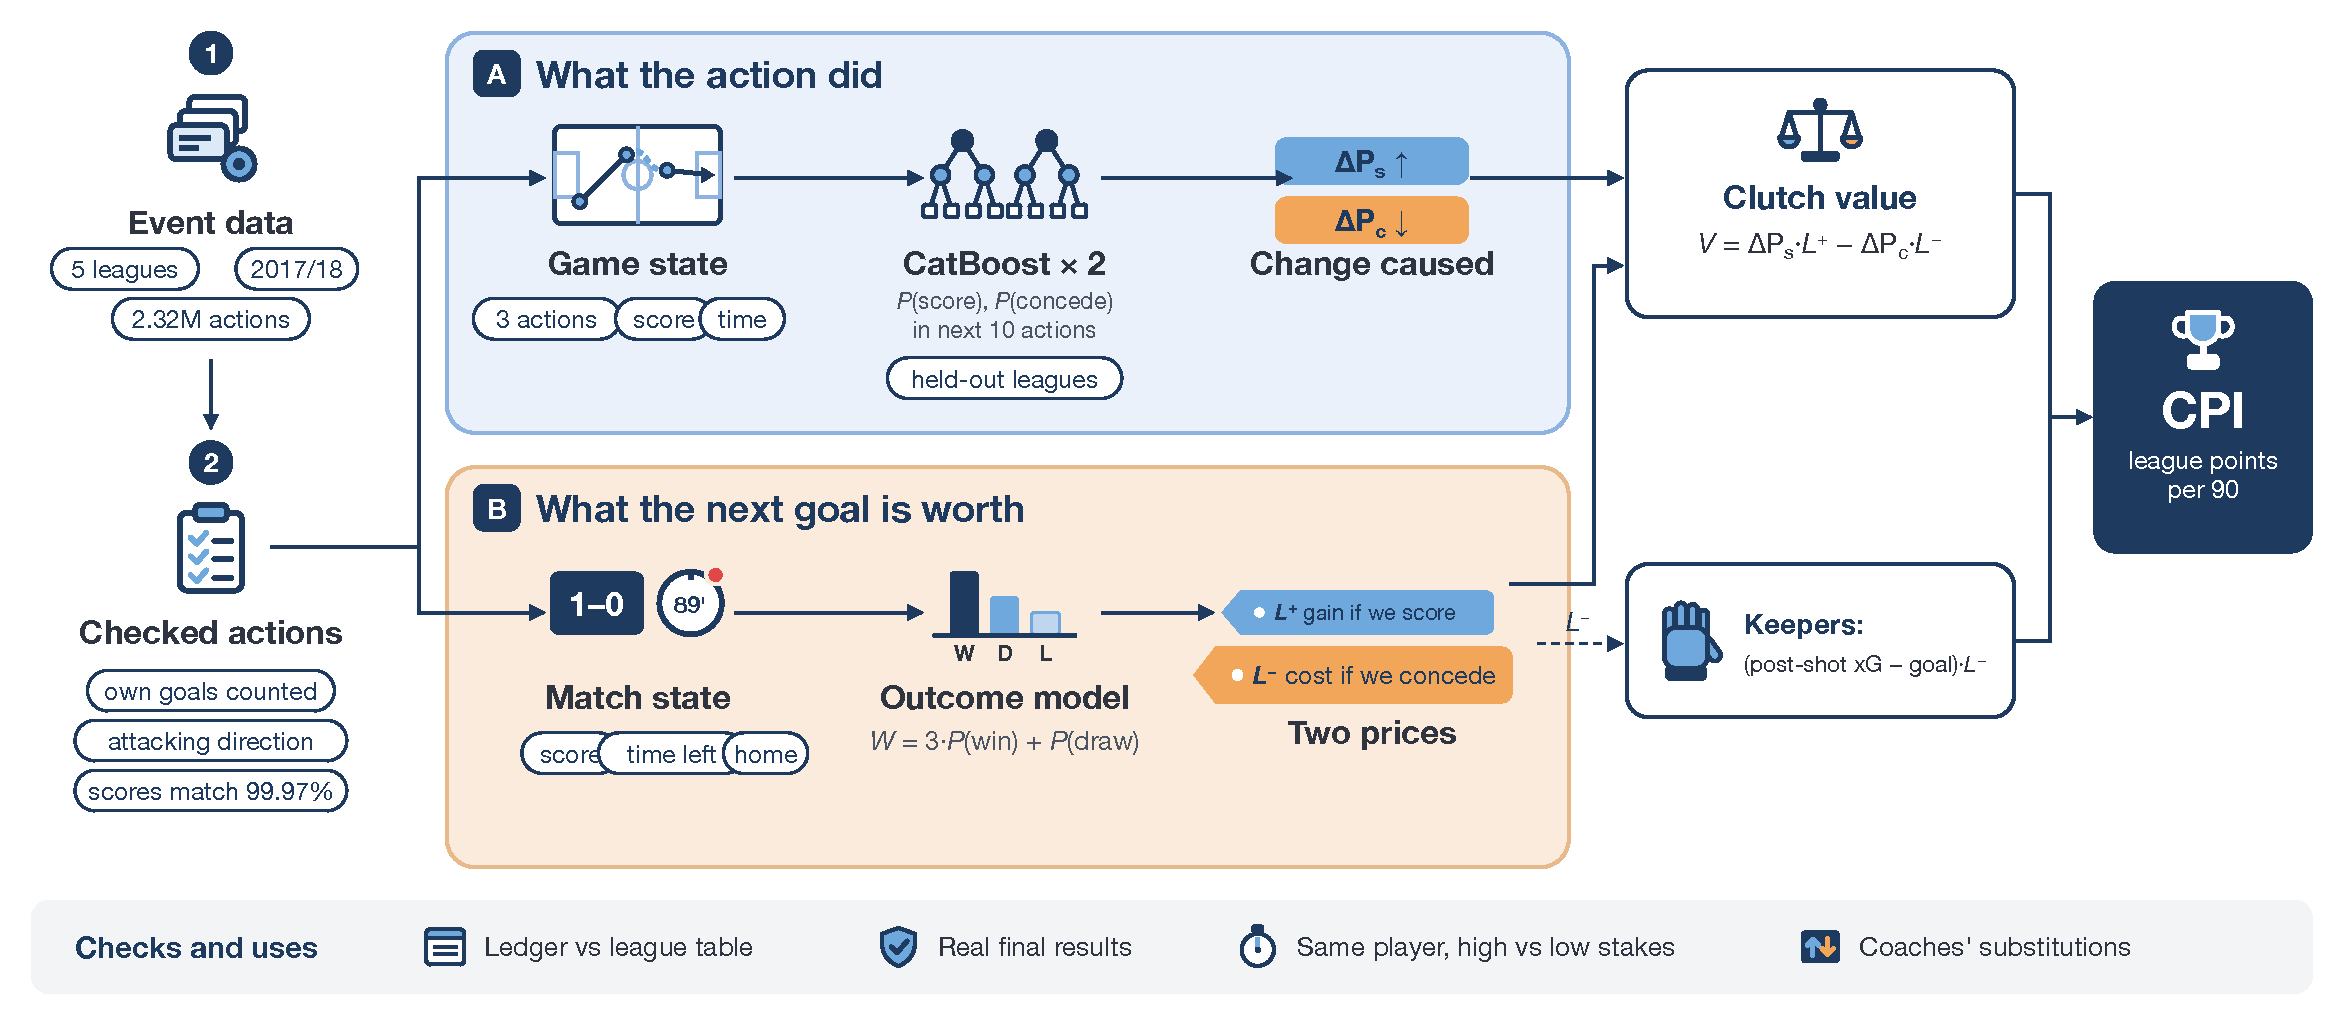
\includegraphics[width=\textwidth]{figures/method.pdf}
\caption{The Clutch Performance Index. Branch A estimates probability changes; branch B estimates scoring and conceding stakes. Their weighted difference gives action value. Player totals, including goalkeeper shot-stopping, are normalised per 90 minutes.}
\label{fig:method}
\end{figure}

\subsection{Estimating What an Action Changes}
\label{sec:actionchanges}
For each action, two CatBoost models estimate the acting team's probabilities of scoring and conceding within the next 10 actions, counting the current action. The corresponding training labels capture these two outcomes separately, with own goals attributed to the opposing team. Both models use \nFeatures{} features describing the current action, its two predecessors, their locations and outcomes, and the match score and time. Evaluated on held-out leagues, the models achieve ROC-AUC scores of \aucScores{} for scoring and \aucConcedes{} for conceding.

Following VAEP~\cite{decroos2019}, we evaluate an action by measuring how it changes the team's probabilities of scoring and conceding between two consecutive game states. Let $P_{s,i}$ and $P_{c,i}$ represent the probabilities of scoring and conceding, respectively, after action $i$. Similarly, $P_{s,i-1}$ and $P_{c,i-1}$ represent these probabilities after the preceding action. All probabilities are considered from the perspective of the team performing action $i$. The changes are
\begin{equation}
\Delta P_{s,i}=P_{s,i}-P_{s,i-1},\qquad
\Delta P_{c,i}=P_{c,i}-P_{c,i-1}.
\end{equation}
VAEP calls $\Delta P_{s,i}$ the action's \textit{offensive value} and $-\Delta P_{c,i}$ its \textit{defensive value}. For example, increasing the estimated scoring chance from 10\% to 15\% gives an offensive value of 0.05, a rise of five percentage points. Reducing the conceding chance gives a positive defensive value.

The preceding probabilities are adjusted at changes in play, following the socceraction implementation~\cite{socceraction}. When the acting team changes, the scoring and conceding predictions from the preceding state swap roles. After a goal or a gap over 10\,s, both are set to zero. We also apply the goal reset to own goals. Penalties and corners use fixed scoring probabilities before the set piece, so takers are credited for execution rather than for obtaining the opportunity. The first action is assigned zero change, as no preceding action is available.

\subsection{Measuring What the Next Goal Is Worth}
An outcome model uses the current score, time remaining and home--away status to predict the number of goals each team is expected to score and, in turn, estimate the probabilities of winning or drawing. Following~\cite{kharrat2020}, team strength is left out: the action values already reflect player quality, so including it would count that quality twice and give players in strong teams less credit for the same action. The model specification is in Appendix~\ref{app:stakes}. Let $g$ be the team's goals minus its opponent's goals. A win earns three league points and a draw one, so expected points at the current time and home--away status are
\begin{equation}
W(g)=3P(\mathrm{win}\mid g)+P(\mathrm{draw}\mid g).
\end{equation}
We denote the expected gain from scoring by $\Lp$ and the expected cost of conceding by $\Lm$. Scoring raises the goal difference by one and conceding lowers it by one, giving
\begin{equation}
\Lp(g)=W(g{+}1)-W(g),\qquad
\Lm(g)=W(g)-W(g{-}1).
\end{equation}
We hold time, home--away status and forecast scoring rates fixed across these scenarios to isolate the effect of the score change.

\subsection{From Action Values to Player Ratings}
We combine each action's probability changes with its pre-action stakes to obtain its clutch value, $V_i$. For player $p$, $A_p$ contains the player's actions and $\text{minutes}_p$ is the total playing time. Summing the on-ball values and scaling by playing time gives CPI per 90 minutes as below:
\begin{equation}
\begin{aligned}
V_i&=\Delta P_{s,i}\,\Lp_i-\Delta P_{c,i}\,\Lm_i,\\
\mathrm{CPI}_p&=\frac{90}{\text{minutes}_p}\sum_{i\in A_p}V_i.
\end{aligned}
\end{equation}
Thus, CPI weights VAEP's offensive value by the gain from scoring, $\Lp$, and its defensive value by the cost of conceding, $\Lm$. Reducing the conceding chance makes the second term positive and earns preventive credit. CPI expresses both contributions in league points per 90 minutes. Rankings compare \nQualified{} players with at least 900 minutes within position~\cite{bransen2019}.

\subsection{Accounting for Goalkeeper Saves}
The shot's outcome already enters the action predictions, which can leave little credit for the subsequent save event. We therefore remove save-event values from the keeper's on-ball total and add a separate shot-stopping estimate, while other actions retain their values. For each on-target shot, $x_{\text{post}}$ estimates the chance of a goal from its location, type and goal-mouth zone. The outcome $\text{goal}$ is 1 if scored and 0 otherwise. $\Lm_{\text{keeper}}$ is the cost of conceding for the keeper's team before the shot. The keeper's total points saved are described as:
\begin{equation}
\text{points saved}=\textstyle\sum_{\text{shots}}(x_{\text{post}}-\text{goal})\,\Lm_{\text{keeper}}.
\end{equation}
A save earns credit according to the shot's difficulty and the stakes, while goals conceded reduce the total. The adjusted keeper total is divided by playing time and multiplied by 90. Team-level analyses retain the original action totals and omit points saved to avoid double counting.

\subsection{Reporting Uncertainty}
We report 95\% intervals for CPI from 1,000 resamples of whole matches, keeping model predictions fixed~\cite{brill2025}. We also report adjusted ratings from an Empirical-Bayes model, which pull less certain estimates towards the position mean. Top-10 probabilities are calculated using these adjusted ratings, whereas the 95\% intervals are based on unadjusted CPI. We report these separately because conventional bootstrap methods can produce inconsistent estimates of rank uncertainty~\cite{hall2009}.

\section{Empirical Validation of CPI}
\label{sec:stakes}
We first examine whether the scoring and conceding stakes reflect observed match consequences, then check how aggregated action values relate to team results.

\subsection{Consequences of Scoring and Conceding}
We estimate gains from scoring and costs of conceding by comparing final league points across adjacent score states, adjusting for pre-match Elo difference~\cite{hvattum2010} and home advantage. After the 80th minute, a team leading by one goal faces an estimated conceding cost of \realCost{} points and a scoring gain of only \realGain{} (difference \costGainDiff{}, 95\% interval \costGainLow{} to \costGainHigh{}). In soccer terms, a late equaliser takes away most of the two points that separate a win from a draw, while a second goal adds little to a win that is already likely.

The model follows these observed consequences across \nCells{} combinations of score state and 10-minute bin (Fig.~\ref{fig:stakes}), with mean absolute errors of about \maeCost{} points for both gains and costs. Scoring-only pressure tracks the gains well, but its Spearman correlation with conceding costs is only \rhoCostSO{}, compared with \rhoCost{} for $\Lm$. The observed asymmetry therefore supports valuing prevention separately from attack.

\begin{figure}[htbp]
\centering
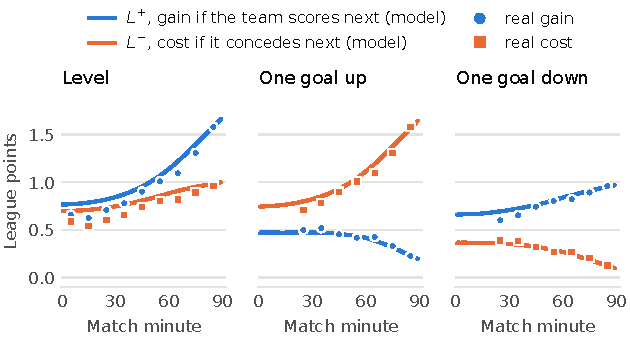
\includegraphics[width=\textwidth]{figures/stakes.pdf}
\caption{Scoring gains and conceding costs over match time. Lines are model estimates for held-out leagues; points are contrasts in observed final points, adjusted for Elo difference and home advantage.}
\label{fig:stakes}
\end{figure}

\subsection{Agreement with Team Results}
We next sum each team's action values and subtract its opponent's total. At match level, this net value follows the points earned more closely than the goal difference itself does (Pearson correlation \ledgerMatchR{} against \ledgerMatchRGd{}), reflecting that the stakes weight each goal by whether it changes a win, draw or defeat. Across \ledgerTeams{} team seasons, the correlation is \ledgerSeasonR{} with a slope of \ledgerSeasonSlope{} (Fig.~\ref{fig:ledger}). Clutch values are therefore on the scale of league points -- a CPI of 0.3 corresponds to about 0.3 points per 90 minutes.

\begin{figure}[htbp]
\centering
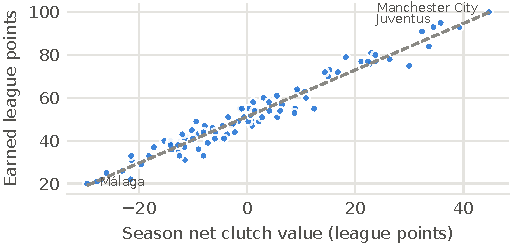
\includegraphics[width=0.85\textwidth]{figures/season_points.pdf}
\caption{Season net clutch value against earned league points, one dot per team. The dashed fitted line includes an intercept.}
\label{fig:ledger}
\end{figure}

\FloatBarrier
\section{How Match Context Changes Player Assessment}
\label{sec:cpi}
For player assessment, the central question is how much an action mattered to the result. We first consider goals, then the preventive actions and saves that protect a lead, and finally who delivered most.

\subsection{Credit for Decisive Actions}
A late winner can turn one point into three, whereas another goal in a comfortable win changes little about the result. VAEP gives both kinds of goal similar values, because it measures the change in scoring chance, which is much the same for most goals (Table~\ref{tab:goals}). CPI separates them: a goal at level scores after the 85th minute is worth \goalLevelLateV{} league points on average, while a goal three or more ahead after the 60th minute is worth almost nothing. The same shift holds across all actions. The lowest-stakes 20\% of actions account for \shareLowVaep\% of total absolute VAEP value but only \shareLowCpi\% of total absolute CPI value. Conversely, the highest-stakes 20\% account for a larger share of total absolute CPI value (\shareTopCpi\%) than of total absolute VAEP value (\shareTopVaep\%). For match review, CPI therefore directs attention to the contributions that shaped the result, while VAEP continues to describe their quality.

\begin{table}[htbp]
\centering
\caption{Mean values of non-penalty goals by match context. VAEP is on a goal-probability scale; $V$ is in league points.}
\label{tab:goals}
\small
\setlength{\tabcolsep}{6pt}
\begin{tabular}{@{}lrcc@{}}
\toprule
Goal scored when & Count & VAEP & $V$ \\
\midrule
\tabGoalValues
\bottomrule
\end{tabular}
\end{table}

\subsection{Scoring Value Beyond Goal Totals}
Goal totals tell us how often a player scored; Fig.~\ref{fig:goals} also shows how much those goals mattered. The dashed line marks the average value per goal, so players above it scored when results were more at stake than usual, and players below it scored more of their goals at low stakes. Moreno, well above the line, matches Ronaldo's season scoring value with \goalsMoreno{} goals to Ronaldo's \goalsRonaldo{}. A scout reading only the scoring chart would miss this difference. Goals, however, are only part of the picture. CPI also credits the actions that stop them.

\begin{figure}[htbp]
\centering
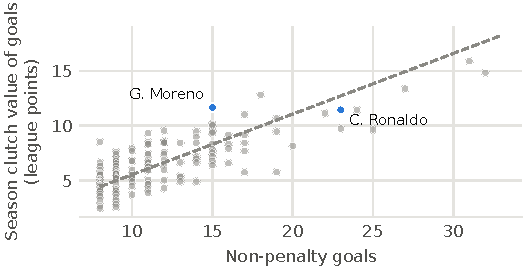
\includegraphics[width=0.85\textwidth]{figures/goals_context.pdf}
\caption{Non-penalty goal totals and their estimated season clutch value, for players with at least eight such goals. The dashed line marks the sample's average value per goal. Totals cover goals only; CPI also includes other actions and is scaled per 90 minutes.}
\label{fig:goals}
\end{figure}

\subsection{Credit for Protecting a Lead}
Protecting a lead is another form of decisive performance. A clearance that reduces the threat of a late equaliser helps preserve the win even though it adds no goal or assist. In \exBMatch{}, with the home side leading \exBScore{} in minute \exBMinute{}, a clearance by \exBPlayer{} cut the estimated chance of conceding from \exBPrevPc{} to \exBPc{}. Because conceding would then have cost \exBLm{} league points, CPI values the clearance at \exBV{} points, against \exBVaep{} under VAEP. Across all moments when a team is ahead, preventive actions receive \creditLow{} to \creditHigh{} times the credit that scoring-only pressure would give them, once both weightings are put on the same average scale.

For a goalkeeper, a save's match value also depends on what conceding would cost. David de Gea prevented more estimated goals than Jan Oblak, yet their points-saved totals are nearly equal (\savedGea{} and \savedOblak{}), because Oblak's saves came at higher stakes. CPI thus credits keepers for the results their saves protect, not only for the goals they prevent.

\subsection{Who Delivered When It Mattered}
Table~\ref{tab:profiles} lists the highest CPI in each position. Lionel Messi leads all players with \messiCPI{} league points per 90. The other position leaders include players outside the usual headlines, such as Jérôme Roussillon (Montpellier) in defence and Nick Pope (Burnley) in goal. This is the kind of profile CPI is built to surface: players whose contributions came when results were at stake, whatever their reputation. The table's intervals, adjusted ratings and top-10 probabilities show how firmly each place is held. Messi's lead is the clearest.

\begin{table}[htbp]
\centering
\caption{Highest estimated CPI within each position among players with at least 900 minutes. CPI and Adjusted (Empirical-Bayes CPI) are league points per 90, with 95\% match-bootstrap intervals; Top 10 is the posterior probability of a top-10 place within the position.}
\label{tab:profiles}
\small
\setlength{\tabcolsep}{6pt}
\begin{tabular}{@{}llccc@{}}
\toprule
Position & Player & CPI (95\% interval) & Adjusted & Top 10 \\
\midrule
\tabProfilesFull
\bottomrule
\end{tabular}
\end{table}

\FloatBarrier
\section{Attacking and Preventive Value in Substitution Choices}
\label{sec:football}
\label{sec:coaches}
Picture a team leading 1--0 with fifteen minutes left. The manager must decide who comes off and who comes on, and the right answer depends on the scoreline: a lead needs protecting, a deficit needs a goal. CPI draws the same line by valuing attacking and preventive contributions separately. Substitution decisions therefore provide an opportunity to examine whether coaches' choices reflect the demands of the scoreline.

We study the \nTakenOff{} coming-off and \nBroughtOn{} coming-on decisions made from the 60th minute with a team one goal up or down. Each candidate's attacking and goal-prevention ratings come from their other matches, so the game being decided does not influence their ratings, and candidates are compared within each substitution decision.

\begin{figure}[htbp]
\centering
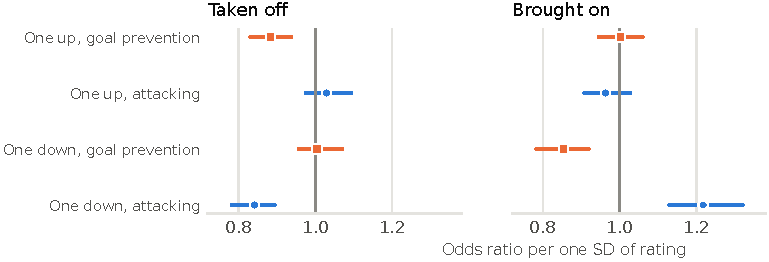
\includegraphics[width=\textwidth]{figures/coaches.pdf}
\caption{Substitution choices and CPI's two components (\nTakenOff{} coming-off and \nBroughtOn{} coming-on decisions). Blue marks the attacking rating and orange the goal-prevention rating. Odds ratios are per standard deviation of rating from other matches; values below 1 mean lower odds of selection. Bars are 95\% match-bootstrap intervals. Leading and trailing reverse which component matters.}
\label{fig:coaches}
\end{figure}

\textbf{Coaches Keep the Players the Scoreline Needs.} When protecting a lead, a player whose goal-prevention rating is one standard deviation higher has about \pctOffUpDef\% lower odds of being taken off, while attacking quality makes no clear difference (Fig.~\ref{fig:coaches}). When chasing, the roles reverse. Stronger attackers have about \pctOffDownAtt\% lower odds of coming off, and prevention makes no clear difference. A holding midfielder who cuts out passes is worth keeping at 1--0, a forward who creates chances at 0--1, and coaches' decisions follow that logic. The reversal is statistically significant (Table~\ref{tab:swap}). A single overall rating, which mixes the two components, cannot show it.

\begin{table}[htbp]
\centering
\caption{Change in each component's odds ratio from trailing by one to leading by one (ratio of odds ratios), with 95\% intervals and two-sided $p$ values from 500 match resamples.}
\label{tab:swap}
\small
\setlength{\tabcolsep}{6pt}
\begin{tabular}{@{}llcc@{}}
\toprule
Decision & Component & Ratio (95\% interval) & $p$ \\
\midrule
\tabSwap
\bottomrule
\end{tabular}
\end{table}

\textbf{The Bench Tells a Different Story.} When chasing a deficit, coaches show a preference for their strongest attacking options: the highest-rated attacker on the bench is brought on in \pickDownR\% of decisions, compared with \pickDownChanceR\% under a rating-independent selection benchmark. When protecting a lead, however, the highest-rated goal preventer is brought on in \pickUpR\% of decisions, matching the expected rate under the same benchmark. Thus, although coaches tend to retain players with stronger goal-prevention ratings when protecting a lead, they do not show a similar preference when selecting substitutes. Analysts can therefore use the two components to review late-game substitutions, and the goal-prevention rating to shortlist bench players for protecting a lead.

\section{Robustness and Repeatability}
\label{sec:robust}
\noindent\textbf{Modelling Choices.} CPI rankings are highly stable across several modelling choices. Within-position rank correlations remain at or above \sensRhoMin{} when changing the random seed, gradient-boosting model, prediction window or inclusion of team strength in the stakes. Data conventions have a greater effect. Incorrectly accounting for attacking direction in away-team actions misplaces shots, reducing scoring ROC-AUC from \baseAuc{} to \mirrorAuc{} and changing mean goalkeeper CPI from \baseKeeper{} to \mirrorKeeper{}. Removing the penalty and corner adjustments increases mean forward CPI from \baseForward{} to \noBaseForward{}, as players receive credit for winning set pieces rather than only for their execution. Across these alternative data conventions, rank correlations fall to as low as \choiceRhoMin{}. The pipeline therefore checks attacking direction automatically and applies the set-piece adjustments consistently.

\textbf{Repeatability.} Stability across modelling choices does not necessarily mean that player ratings remain consistent across matches. To examine repeatability, we compare ratings from odd- and even-gameweek halves of the season. Reliability is the Spearman correlation between players' per-90 ratings in the two halves within each position, adjusted to full-season length with the Spearman--Brown correction. CPI shows lower split-half reliability than VAEP across all positions, with the lowest reliability among goalkeepers (Table~\ref{tab:trust}). This difference partly reflects what the two metrics measure. VAEP evaluates the quality of a player's actions, whereas CPI also accounts for when those actions occur and the importance of the match situation. High-stakes situations, such as close matches late in the game, vary across a team's fixtures and results, making CPI more sensitive to the distribution of match situations within each half of the season. CPI therefore reflects the value a player delivered under the circumstances of a particular season, rather than necessarily indicating a consistently repeatable level of performance. The reported intervals and adjusted ratings provide additional information about the uncertainty in these player comparisons.

\begin{table}[htbp]
\centering
\caption{Split-half reliability between odd- and even-gameweek ratings, with the Spearman--Brown correction; players need at least 450 minutes in each half.}
\label{tab:trust}
\small
\setlength{\tabcolsep}{6pt}
\begin{tabular}{@{}lcc@{}}
\toprule
Position & CPI & VAEP \\
\midrule
Forwards & \relCPIF & \relVaepF \\
Midfielders & \relCPIM & \relVaepM \\
Defenders & \relCPID & \relVaepD \\
Goalkeepers & \relCPIG & \relVaepG \\
\bottomrule
\end{tabular}
\end{table}

\FloatBarrier
\section{Discussion and Conclusion}
\label{sec:discussion}
CPI connects action quality with match consequences. Observed outcomes support separate scoring and conceding stakes, and aggregated values track team points. The resulting credit highlights decisive goals and the contributions that protect a result, and coaches' substitutions show that the attacking and preventive components matter at opposite scorelines.

\textbf{Use for Analysts.} An analyst can use CPI and its uncertainty intervals together with VAEP to select consequential contributions for video review. Reviewing clearances and saves from narrow leads next to attacking actions makes prevention visible, and the goal-prevention rating can inform who is sent on to protect a lead.

\textbf{Limitations and Future Work.} The stakes are defined by league points, three for a win and one for a draw. CPI therefore applies directly to leagues and to tournament group stages, but not to knockout matches, where a draw leads to extra time or penalties and two-legged ties depend on the aggregate score. The framework carries over by replacing expected league points with the probability of progressing, estimated from knockout data; developing this version is a natural next step. The study also covers one season of recorded on-ball actions, leaving off-ball work unmeasured, and role, opportunity and tactical instructions shape every rating. CPI is less repeatable than VAEP, which limits claims about a persistent clutch ability; goalkeeper estimates are particularly uncertain, and the intervals exclude uncertainty from model training. The substitution analysis describes choices rather than their effectiveness, stakes weighting does not improve its fit over unweighted components, and ratings from other matches can include later games. Multiple seasons with chronological validation, tracking data for off-ball contributions and prospective tests of substitution advice would address these points.

\textbf{Conclusion.} CPI provides a common league-points scale for examining who delivered valuable attacking, preventive and goalkeeping contributions when results were at stake.

\appendix
\section{Models and Stakes}
\label{app:stakes}
\textbf{Action Values.} For the action and its two predecessors, the \nFeatures{} features cover action type, outcome and body part; start and end locations, distances and angles to goal, and movement; period and time; whether each predecessor belongs to the acting team, with the time and distance since it; and the acting team's goals, the opponent's goals and their difference. All locations follow the acting team's attacking direction. CatBoost uses up to 1,000 trees (learning rate 0.05, depth 6, $\ell_2$ regularisation 3, log-loss) with early stopping on 15\% of training matches. Across the five held-out leagues, ROC-AUC ranges from \foldAucS{} for scoring and from \foldAucC{} for conceding, and expected calibration error is at most \eceMax{}$\times10^{-3}$. Following socceraction, the scoring probability before penalties and corners is fixed at 0.792 and 0.047.

\textbf{Outcome Model.} A match is divided into 100 intervals of 54 seconds. With goal difference $g$, intervals remaining $n$ and home indicator $h$, the chance of scoring at least once more is $f(g,n,h)=\sigma(\beta_0+\beta_g g+\beta_n n+\beta_{nn}n^2+\beta_h h)$, fitted by $\ell_2$-regularised logistic regression with one row per team and interval. Richer forms with red cards or score-by-time interactions did not improve the held-out ranked probability score by the 0.5\% required in advance. The chance becomes a per-interval rate $\theta=1-(1-f)^{1/n}$, and the opponent's rate uses $f(-g,n,1-h)$. With independent future goals $U\sim\mathrm{Bin}(n,\theta^+)$ and $D\sim\mathrm{Bin}(n,\theta^-)$,
\begin{equation}
P(\mathrm{win}\mid g)=\sum_{u=0}^{6}\sum_{d=0}^{6}b(u;n,\theta^+)\,b(d;n,\theta^-)\,\mathbf 1[g+u-d>0],
\end{equation}
where $b$ is the binomial probability; $P(\mathrm{draw}\mid g)$ uses $\mathbf 1[g+u-d=0]$. Rates and time stay fixed when evaluating $g\pm1$.

\textbf{Goalkeepers and Uncertainty.} The post-shot model is a gradient-boosted classifier on the \psxgShots{} on-target shots, using start location, distance, angle, a header flag, shot type and goal-mouth zone. Trained on four leagues and tested on the fifth, its ROC-AUC is \psxgAuc{}, with \psxgPred{} goals predicted against \psxgGoals{} scored. Intervals come from 1,000 match resamples with predictions fixed. Within each position, the Empirical-Bayes rating is $w_px_p+(1-w_p)\mu$ with $w_p=\tau^2/(\tau^2+s_p^2)$, where $s_p^2$ is the bootstrap variance of rating $x_p$, $\tau^2$ the between-player variance and $\mu$ the precision-weighted position mean. Top-10 probabilities use 20,000 draws from $\mathcal N(w_px_p+(1-w_p)\mu,\,w_ps_p^2)$.

\section{Substitution Analysis}
\label{app:designs}
For each substitution from minute 60 at goal difference $\pm1$, the candidates are the eligible outfield players on the pitch (coming off) or on the unused bench (coming on), each with at least 450 minutes in other matches. A conditional logit model compares candidates within each decision using their standardised attacking and goal-prevention ratings, position and, for players coming off, time on the pitch and a yellow card. Intervals use 500 match resamples. Table~\ref{tab:swap} reports how each component's association changes between scorelines.

\FloatBarrier
\begin{credits}
\subsubsection{\discintname}
The authors have no competing interests to declare that are relevant to the content of this article.
\end{credits}

\begin{thebibliography}{13}
\raggedright
\bibitem{decroos2019} Decroos, T., Bransen, L., Van Haaren, J., Davis, J.: Actions speak louder than goals: valuing player actions in soccer. In: Proc. 25th ACM SIGKDD, pp. 1851--1861 (2019). \doi{10.1145/3292500.3330758}
\bibitem{bransen2019} Bransen, L., Robberechts, P., Van Haaren, J., Davis, J.: Choke or shine? Quantifying soccer players' abilities to perform under mental pressure. In: MIT Sloan Sports Analytics Conference (2019)
\bibitem{robberechts2021} Robberechts, P., Van Haaren, J., Davis, J.: A Bayesian approach to in-game win probability in soccer. In: Proc. 27th ACM SIGKDD, pp. 3512--3521 (2021). \doi{10.1145/3447548.3467194}
\bibitem{deshpande2016} Deshpande, S.K., Jensen, S.T.: Estimating an NBA player's impact on his team's chances of winning. J. Quant. Anal. Sports \textbf{12}(2), 51--72 (2016). \doi{10.1515/jqas-2015-0027}
\bibitem{kharrat2020} Kharrat, T., McHale, I.G., L\'opez Pe\~na, J.: Plus--minus player ratings for soccer. Eur. J. Oper. Res. \textbf{283}(2), 726--736 (2020). \doi{10.1016/j.ejor.2019.11.026}
\bibitem{otten2009} Otten, M.: Choking vs. clutch performance: a study of sport performance under pressure. J. Sport Exerc. Psychol. \textbf{31}(5), 583--601 (2009). \doi{10.1123/jsep.31.5.583}
\bibitem{swann2017} Swann, C., Crust, L., Jackman, P., Vella, S.A., Allen, M.S., Keegan, R.: Performing under pressure: exploring the psychological state underlying clutch performance in sport. J. Sports Sci. \textbf{35}(23), 2272--2280 (2017). \doi{10.1080/02640414.2016.1265661}
\bibitem{franks2016} Franks, A., D'Amour, A., Cervone, D., Bornn, L.: Meta-analytics: tools for understanding the statistical properties of sports metrics. J. Quant. Anal. Sports \textbf{12}(4), 151--165 (2016). \doi{10.1515/jqas-2016-0098}
\bibitem{brill2025} Brill, R.S., Yurko, R., Wyner, A.J.: Exploring the difficulty of estimating win probability: a simulation study. J. Quant. Anal. Sports \textbf{22}(1), 105--115 (2026). \doi{10.1515/jqas-2024-0130}
\bibitem{hall2009} Hall, P., Miller, H.: Using the bootstrap to quantify the authority of an empirical ranking. Ann. Statist. \textbf{37}(6B), 3929--3959 (2009). \doi{10.1214/09-AOS699}
\bibitem{pappalardo2019} Pappalardo, L., et al.: A public data set of spatio-temporal match events in soccer competitions. Sci. Data \textbf{6}, 236 (2019). \doi{10.1038/s41597-019-0247-7}
\bibitem{socceraction} Decroos, T., et al.: socceraction, version 1.5.3. \url{https://github.com/ML-KULeuven/socceraction}, last accessed 2026/11/13
\bibitem{hvattum2010} Hvattum, L.M., Arntzen, H.: Using ELO ratings for match result prediction in association football. Int. J. Forecast. \textbf{26}(3), 460--470 (2010). \doi{10.1016/j.ijforecast.2009.10.002}
\end{thebibliography}

\end{document}
